This report summarizes the achievements in Work Package 6 over the last year of the OpenDreamKit project\footnote{By oversight the title in the grant agreement has not been updated} Concretely, this report reports on the results of \tasktref{dksbases}{mws} and \tasktref{dksbases}{isabelle} and tasks \taskref{dksbases}{data-OEIS} to \taskref{dksbases}{data-LMFDB} (case studies in mathematical data sets).

In the last year, significant progress has been made in four areas, which we will introduce in the next subsections (\ref{sec:tetrapod} to \ref{subsec:software}) and then detail the latter three in the corresponding Sections~\ref{sec:knowledge} to \ref{sec:software}.

\subsection{A New Conceptual Model for Mathematical VREs}\label{sec:tetrapod}
The probably most fundamental progress for a mathematical research environment is a new understanding of the aspects of virtual research environments reached via the intensive work with the semantics of VREs in \WPref{dksbases}.  We have codified the experiences in the OpenDreamKit project into a tetrapodal view on ``doing
mathematics'' -- i.e. the activity to be supported by a VRE.

We propose that all mathematical VREs need to support the following four main aspects at scale:
\begin{compactenum}[\em i\rm)]
\item \textbf{Inference}: deriving statements by \emph{deduction} (i.e.,
  proving), \emph{abduction} (i.e., conjecture formation from best
  explanations), and \emph{induction} (i.e., conjecture formation from examples).
\item \textbf{Computation}: algorithmic manipulation and simplification
  of mathematical expressions and other representations of
  mathematical objects.
\item \textbf{Tabulation}: generating, collecting, maintaining, and accessing
  collections of examples that suggest patterns and relations and allow testing
  of conjectures. 
\item \textbf{Narration}: bringing the results into a form that can be digested by humans,
  usually in mathematical documents like articles, books, or preprints, that expose the
  ideas in natural language but also in diagrams, tables, and simulations.
\end{compactenum} 
Computer support exists for all of these four aspects of Big Math, e.g.,
\begin{compactenum}[\em i\rm)]
\item theorem provers like Isabelle, Coq, or Mizar;
\item computer algebra systems like GAP, SageMath, Maple, or Mathematica; and
\item mathematical data bases like the L-functions and Modular Forms Data 
Base (LMFDB)~\cite{Cremona:LMFDB16,lmfdb:on} and the Online Encyclopedia of
Integer Sequences (OEIS)~\cite{Sloane:OEIS};
\item online journals, mathematical information systems like zbMATH or MathSciNet,
  preprint servers like arXiv.org, or research-level help systems like MathOverflow.
\end{compactenum}
Humans can easily integrate these four aspects and do that for all mathematical developments, the corresponding integration in software systems is still a significant problem. It is our experience from the \pn project that one of the prerequisites is a \textbf{modular organization} of all four aspects in terms of a joint \textbf{mathematical ontology} -- the Math-in-the-Middle (MitM) ontology introduced in \WPref{dksbases} of the \pn project.

\begin{figure}[ht]\centering
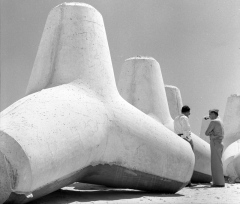
\includegraphics[width=5cm]{tetrapod}\qquad
\documentclass{standalone}
\usepackage{tikzinput}
\begin{document}
\providecommand\myscale{4.5}
\begin{tikzpicture}[scale=\myscale]
  \node (center) at (0,.15) {Organization};
  \node (left) at (.2,-.3) {Computation};
  \node (right) at (.4,0) {Tabulation};
  \node (back) at (-.5,0) {Inference};
  \node (up) at (0,.5) {Narration};

  \draw[very thick] (center) -- (left);
  \draw[very thick] (center) -- (right);
  \draw[very thick] (center) -- (back);
  \draw[very thick] (center) -- (up);
  \draw[dotted] (left) -- (right) -- (back) -- (left);
  \draw[dotted] (up) -- (left);
  \draw[dotted] (up) -- (right);
  \draw[dotted] (up) -- (back);
\end{tikzpicture}
\end{document}
%%% Local Variables: 
%%% mode: latex
%%% TeX-master: t
%%% End: 

\caption{Five Aspects of Math VREs, a Tetrapod Structure}\label{fig:tetrapod}
\end{figure}

\def\hateq{\ensuremath{\widehat=}\xspace} Figure~\ref{fig:tetrapod} organizes these four aspects into a tetrapodal structure with the MitM ontology.  This model extends and refines he Data/Knowledge/Software model of the proposal by ``narration'' and ``organization'' aspects (Data (D) \hateq Tabulation, Knowledge (K) \hateq Inference, and Software (S) \hateq Computation). For details and a discussion in terms of ``big math'' developments like the classification of finite simple groups, consult~\cite{CarFarKohRab:bmobb19}.

The tetrapod model is consistent with the \pn structure and organization: the software aspect is mostly covered by \WPtref{hpc} and \WPtref{component-architecture} in \pn, where the latter develops the aspect of modular \textbf{organization} of the software. \WPtref{UI} covers the interaction between \textbf{Narration} and \textbf{Software} -- again, one of the innovations in the Jupyter framework concerns the modular \textbf{Organization} of software interfaces. \textbf{Inference} and \textbf{Tabulation} are covered in \WPtref{dksbases}.

We will now introduce three aspects that have been studied in detail in \pn in the last year and make up the technical bulk of this report in the sections after this one.  

%%% Local Variables:
%%% mode: latex
%%% mode: visual-line
%%% fill-column: 5000
%%% TeX-master: "report"
%%% End:

%  LocalWords:  WPref dksbases tetrapodal textbf emph Cremona:LMFDB16,lmfdb:on zbMATH organization centering includegraphics qquad hateq ensuremath widehat xspace CarFarKohRab:bmobb19 WPtref hpc WPtref WPtref Jupyter WPtref

\subsection{Formal Knowledge Bases}\label{sec:isabelle}
For the Knowledge (K) aspect (see \textbf{Inference} in Figure~\ref{fig:tetrapod}) we have developed an exporter from library the Isabelle Theorem prover (Archive of Formal Proof) to an extensive RDF triple store, which can be queried by standard SPARQL queries for semantic search.
  
For many decades, the development of a universal database of all mathematical knowledge, as envisioned, e.g., in the QED manifesto \cite{qed}, has been a major driving force of computer mathematics.
Today a variety of such libraries are available.
These are most prominently developed in proof assistants such as Coq \cite{coq} or Isabelle \cite{isabelle} and are treasure troves of detailed mathematical knowledge.
However, despite the enormous potential for many applications of and in virtual research environments, this treasure is usually locked into system- and logic-specific representations that can only be understood by the respective theorem prover system.
For example, this precludes applications such as finding related object in knowledge bases from within computation-oriented systems as used in OpenDreamKit.

Therefore, we have developed interface standards that allow maintainers of formal libraries to make their content available to outside systems.
In this deliverable, we report on complementing our existing OMDoc/MMT standard for representing entire knowledge bases with a new Upper Library Ontology (ULO).
ULO is a standard ontology for exchanging high-level information about mathematical libraries that systematically abstracts all symbolic knowledge away and only retain what can be easily represented relationally.
That allows for semantic web-style representations, for which simple and standardized formalisms such as OWL2 \cite{w3c:owl2-xml}, RDF \cite{rdf}, and SPARQL~\cite{w3c:SPARQL-Rec:13} as well as highly scalable tools are readily available.
While it is well-known that ontology language--based relational formalisms are inappropriate for symbolic knowledge like formulas, algorithms, and proofs, it is this high-level information that is often critically important for integration into virtual research environments, e.g., to realize benefits like search.

We report on this in Section~\ref{sec:knowledge}.
The bulk of this section is taken by a report on the new task (\tasktref{dksbases}{isabelle}) that we have added to \pn in the last amendment of the grant agreement.
In this task, we export the large Isabelle knowledge bases as both OMDoc/MMT and ULO format, resulting in datasets in the double-digit GB range.
We show the utility of the generated ULO data by setting up a relational query engine that provides easy access to certain library information that was previously hard or impossible to determine.

\paragraph{Relational Datasets}
Many mathematical datasets take the form of large SQL/CSV--style datasets that enumerate all or a selection of interesting objects satisfying certain properties, e.g., all finite groups up to a certain size.
These can be produced in bulk or grow from individual user submissions.

They are generally produced, published, and maintained with virtually no systematic attention to the FAIR principles~\cite{FAIR,WilDumAal:FAIR16} for making data findable, accessible, interoperable, and reusable.
In fact, often the sharing of data is an afterthought --- see~\cite{Bercic:cmo:wiki} for an overview of mathematical datasets and their ``FAIR-readiness''.

Moreover, the inherent complexity of mathematical data makes it very difficult to share in practice: even freely accessible datasets are often very hard or impossible to reuse, let alone make machine-interoperable because there is no systematic way of specifying the relation between the raw data and its mathematical meaning. 
Therefore, unfortunately, FAIR mathematical datasets essentially do not exist today.


%%% Local Variables:
%%% mode: latex
%%% mode: visual-line
%%% fill-column: 5000
%%% TeX-master: "report"
%%% End:

%  LocalWords:  textbf standardized rdf tasktref dksbases

\subsection{Mathematical Libraries}\label{sec:mathlib}
% Innovations based on mathematical knowledge and algorithms yield many improvements in science, engineering, economy, ecology, health care, security, and society overall. 
% For example, our global positioning system (GPS) needs the mathematics of relativistic physics, our mobile phones use frequencies allocated through combinatorial optimization, the combinatorics of our genome yields clues to curing rare diseases, the privacy of our communications depends on cryptographic protocols steeped in number theory, and our national security is relying on the mathematical analysis of increasingly complex networks. 
% Fundamental mathematical research and its direct application in practical situations enable many engineering, science, and business innovations that enrich society and mankind.\ednote{FR: throw out this paragraph? Or replace with one sentence?}

% Modern mathematical research increasingly depends on collaborative tools, computational environments, and online databases, and these are changing the way mathematical research is conducted and how it is turned into applications.
% For example, engineers now use mathematical tools to build and simulate physical models based on systems of differential equations with millions of variables, combining building blocks and algorithms taken from libraries shared all over the internet.


For the the data (D) aspect of ``doing mathematics'' (see the \textbf{Tabulation} corner in Figure~\ref{fig:tetrapod}) we have
\begin{compactenum}
\item developed an both an innovative model of (deep) FAIR in mathematics (and have integrated it with the MitM paradigm developed in OpenDreamKit),
\item have implemented in a prototypical system (\dmh), and have
\item evaluated it on the mathematical community outside the core OpenDreamKit community.
\end{compactenum}

Traditionally, mathematics has not paid particular attention to the creation and sharing of data --- the careful computation and publication of logarithm tables is a typical example of the extent and method.
This has changed with the advent of computer-supported mathematics, and the practice of modern mathematics is increasingly data-driven.
Today it is routine to use mathematical datasets in the Gigabyte range, including both human-curated and machine-produced data.
Examples include the L-Functions and Modular Forms Database (LMFDB; $\sim 1$ TB data in number theory)~\cite{Cremona:LMFDB16,lmfdb:on} and the GAP Small Groups Library~\cite{GapSmallGroups:on} with $\sim 450$ million finite groups.  
In a few, but increasingly many areas, mathematics has even acquired traits of experimental sciences in that mathematical reality is ``measured'' at large scale by running computations.

There is wide agreement in mathematics that these datasets should be a common resource and be open and freely available.
Moreover, the software used to produce them is usually open source and free as well.
%While FAIR does not necessarily mean Open~\cite[2.3]{FAIR}, the appropriate Openness for almost all mathematical data is indeed open source and free.
Such an ecosystem is embraced by the mathematics community as a general vision for their future research infrastructure~\cite{NAS14}, adopted by the International Mathematical Union as the Global Digital Mathematics Library initiative \cite{GDML:on}.

To better understand the scale of the problem, Figure~\ref{fig:datasets} gives an overview of some state-of-the-art libraries.
Here we already use the division into four kinds of mathematical data that we will develop in Section~\ref{sec:deep}.

\begin{figure*}[htp]\centering\small\def\cite#1{}
  \begin{tabular}{| p{.35\textwidth} | p{0.55\textwidth}|}\hline
  Dataset & Description \\\hline\hline
  \multicolumn{2}{|l|}{\textbf{Symbolic Knowledge}} \\\hline
  Theorem prover libraries \cite{OAFproject:on}  & $\approx 5$ proof libraries, $\approx 10^5$ theorems each, $\approx 200$ GB \\\hline
  Computer algebra systems \cite{sagemath} & e.g., SageMath distribution bundles $\approx 4$ GB of various tools and libraries\\\hline
  Modelica libraries \cite{Modelica:on} &$> 10$ official, $> 100$ open-source, $\approx 50$ commercial,
      $> 5.000$ classes in the Standard Library, industrial models can reach $.5$M equations \\\hline
  \multicolumn{2}{|l|}{\textbf{Relational Data}} \\\hline
 Integer Sequences \cite{OEIS:on} & $\approx 330$K sequences, $\approx 1$ TB  \\\hline
 Sequence Identities \cite{kwarc:datahost:on} & $\approx .3$M sequence identities, $\approx 2.5$ TB \\\hline
 Highly symmetric graphs, maps, polytopes \cite{ConderCensuses:on, HartleyPolytopes:on, LeemansPolytopes:on, PotocnikCensuses:on, RoyleVT:on, WilsonET:on} & $\approx 30$ datasets, $\approx 2\cdot10^6$ objects, $\approx 1$ TB \\\hline
  Finite lattices \cite{KohLat:on, LeeLat:on, MalLat:on} & $7$ datasets, $\approx 17 \cdot 10^9$ objects, $\approx 1.5$ TB \\\hline
  Combinatorial statistics and maps \cite{findstat} & $\approx1.500$ objects \\\hline
  SageMath databases \cite{SageDB:on} & $12$ datasets \\\hline
  $L$-functions and modular forms \cite{lmfdb:on} & $\approx 80$ datasets, $\approx 10^9$ objects, $\approx 1$ TB \\\hline
  \multicolumn{2}{|l|}{\textbf{Linked Data}} \\\hline
   zbMATH \cite{zbMATH:on} & $\approx 4$M publication records with semantic data, $\approx 30$M reference data, $>1$M disambig. authors, $\approx 2,7$M full text links: $\approx 1$M OA \\\hline
  swMATH \cite{swMATH:on} & $\approx 25$K software records with $> 300$K links to $> 180$K publications \\\hline
  EuDML  \cite{EuDML:on} & $\approx 260$K open full-text publications \\\hline
  Wikidata  \cite{wikidata:on} & $34$ GB linked data, thereof about $4$K formula entities, interlinked, e.g., with named theorems, persons, and/or publications \\\hline
  \multicolumn{2}{|l|}{\textbf{Narrative Data}} \\\hline
  arXiv.org & $\approx 300$K math preprints (of $\approx1.6$M) most with {\LaTeX} sources\\\hline
  EuDML  \cite{EuDML:on} & $\approx 260$K open full-text publications, digitized journal back issues \\\hline
  MathOverFlow & $\approx 1,1$M questions/answers, $\geq11$K answer authors \\\hline
  Stacks project & $\geq 6000$ pages, semantically annotated, curated, searchable textbook \\\hline
    nLab & $\geq 13$K pages on category theory and applications\\\hline
    Jupyter/Sage Notebooks & $\sim10$K public Jupyter notebooks with Sage kernel on GitHub\\\hline
\end{tabular}
  \caption{Summary of mathematical libraries}\label{fig:datasets}
\end{figure*}

We present a uniform infrastructure for sharing, finding, and searching mathematical libraries of any kind.
Moreover, we seed this infrastructure with a collection of representative libraries (all of them state of the art and large) as described below.


%%% Local Variables:
%%% mode: latex
%%% mode: visual-line
%%% fill-column: 5000
%%% TeX-master: "report"
%%% End:

%  LocalWords:  sec:mathlib optimization textbf dmh Cremona:LMFDB16,lmfdb:on centering textwidth textwidth hline OAFproject:on sagemath Modelica Modelica:on ConderCensuses:on LeemansPolytopes:on PotocnikCensuses:on cdot10 cdot lmfdb:on zbMATH zbMATH:on disambig swMATH swMATH:on digitized geq11 geq Jupyter

\subsection{Mixed Computational and Narrative Documents}\label{subsec:software}
Finally, for computational mathematical documents (the S aspect of D/K/S structures from the \pn proposal or the \textbf{narration} and \textbf{computation} aspects of the finer tetrapod model from Figure~\ref{fig:tetrapod}). Here we have developed a formula harvester for Jupyter notebooks and a formula search engine that builds on them (as envisioned in task \taskref{dksbases}{mws}).


\ednote{MK@TW: write summary here, explain selection of example6}

%%% Local Variables:
%%% mode: latex
%%% mode: visual-line
%%% fill-column: 5000
%%% TeX-master: "report"
%%% End:


\subsection{Acknowledgments and Prior Dissemination}
Task D6.10 \ednote{insert task ref} was carried out as a subcontract by Makarius Wenzel.
Some parts of Section~\ref{sec:isabelle} are adapted from his descriptions of his work in the context of this subcontract.

This work has been published as \ednote{cite ULO paper} for ULO.\ednote{add other papers}
The export facilities of Isabelle and the integration with MMT have been integrated with Isabelle in its June 2019 release.
It was reported on in two blog posts by Wenzel%
\footnote{\url{https://sketis.net/2018/isabelle-mmt-export-of-isabelle-theories-and-import-as-omdoc-content}, and \url{https://sketis.net/2019/mmt-as-component-for-isabelle2019}}
and a paper is forthcoming.

%%% Local Variables:
%%% mode: latex
%%% mode: visual-line
%%% fill-column: 5000
%%% TeX-master: "report"
%%% End:

%  LocalWords:  summarizes tasktref dksbases mws tasktref dksbases taskref dksbases taskref dksbases oldpart data.mathhub Jupyter WPref tetrapodal textbf emph Cremona:LMFDB16,lmfdb:on zbMATH organization centering includegraphics qquad hateq ensuremath widehat xspace CarFarKohRab:bmobb19 WPtref hpc WPtref WPtref WPtref sec:mathlib optimization ednote textwidth textwidth hline OAFproject:on sagemath Modelica Modelica:on ConderCensuses:on LeemansPolytopes:on PotocnikCensuses:on cdot10 cdot lmfdb:on disambig swMATH swMATH:on digitized geq11 geq rdf Makarius
